
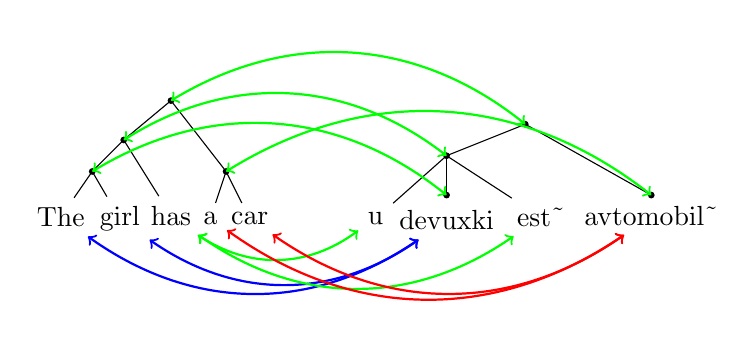
\begin{tikzpicture}

\draw node (the) at (0,0.02) {The};
\draw node (girl) at (0.75,0) {girl};
\draw node (has) at (1.4,0.04) {has};
\draw node (a) at (1.9,0) {a};
\draw node (car) at (2.4,0) {car};
\draw node (y) at (4,0) {\textcyr{u}};
\draw node (girlr) at (4.9,-0.02) {\textcyr{devuxki}};
\draw node (is) at (6.1,0.02) {\textcyr{est\char126}};
\draw node (carr) at (7.5,0.04) {\textcyr{avtomobil\char126}};

\coordinate (thegirl) at (0.4,0.6);
\coordinate (acar) at (2.1,0.6);
\coordinate (thegirlhas) at (0.8,1);
\coordinate (all) at (1.4,1.5);
\coordinate (carr_) at (7.5, 0.3);
\coordinate (girlr_) at (4.9,0.3);
\coordinate (girlhas) at (4.9,0.8);
\coordinate (allr) at (5.9, 1.2);


\foreach \coordinate in {thegirl, acar, thegirlhas,all,carr_, girlr_, girlhas, allr}
	\filldraw (\coordinate) circle (0.035);

\foreach \from/\to in {thegirl/girl, thegirl/the, acar/a, acar/car, thegirlhas/thegirl, thegirlhas/has, all/thegirlhas, all/acar, girlhas/girlr_, girlhas/y, girlhas/is, allr/girlhas, allr/carr_}
	\draw (\from) -- (\to);

\foreach \from/\to in {the/girlr, girl/girlr}
	\draw[<->, bend left = -35, thick, blue] (\from) to (\to);

\foreach \from/\to in {has/y, has/is, allr/all, girlhas/thegirlhas, carr_/acar, girlr_/thegirl}
	\draw[<->, bend left = -35, thick, green] (\from) to (\to);

\foreach \from/\to in {a/carr, car/carr}
	\draw[<->, bend left = -35, thick, red] (\from) to (\to);

\end{tikzpicture}